% CCI v2 -- Counterfactual TEST manifest: "fate per source group" diagram.
% 4 keyword groups -> symmetry-filter verdict (+ rule) -> resulting pairs (bars).
% Numbers code-verified by re-running the swap engine on the 1,060-tweet test
% split: 2,117 pairs (Jews 1,725; Israel 392; Kikes 0; ZioNazi 0).
% Compiles with pdflatex (MiKTeX). Standalone -> tight-cropped PDF.
\documentclass[tikz,border=10pt]{standalone}
\usepackage{amsmath}
\usetikzlibrary{positioning, arrows.meta, backgrounds, calc, shadows.blur, fit}

% ---- Okabe-Ito palette ----
\definecolor{inkdark}{HTML}{1F2937}
\definecolor{accept}{HTML}{009E73}   % green  -> accepted
\definecolor{reject}{HTML}{D55E00}   % vermillion -> rejected
\definecolor{jewsc}{HTML}{0072B2}    % blue
\definecolor{isrc}{HTML}{E69F00}     % gold
\definecolor{slate}{HTML}{6B7280}
\definecolor{rail}{HTML}{E5E7EB}

\begin{document}
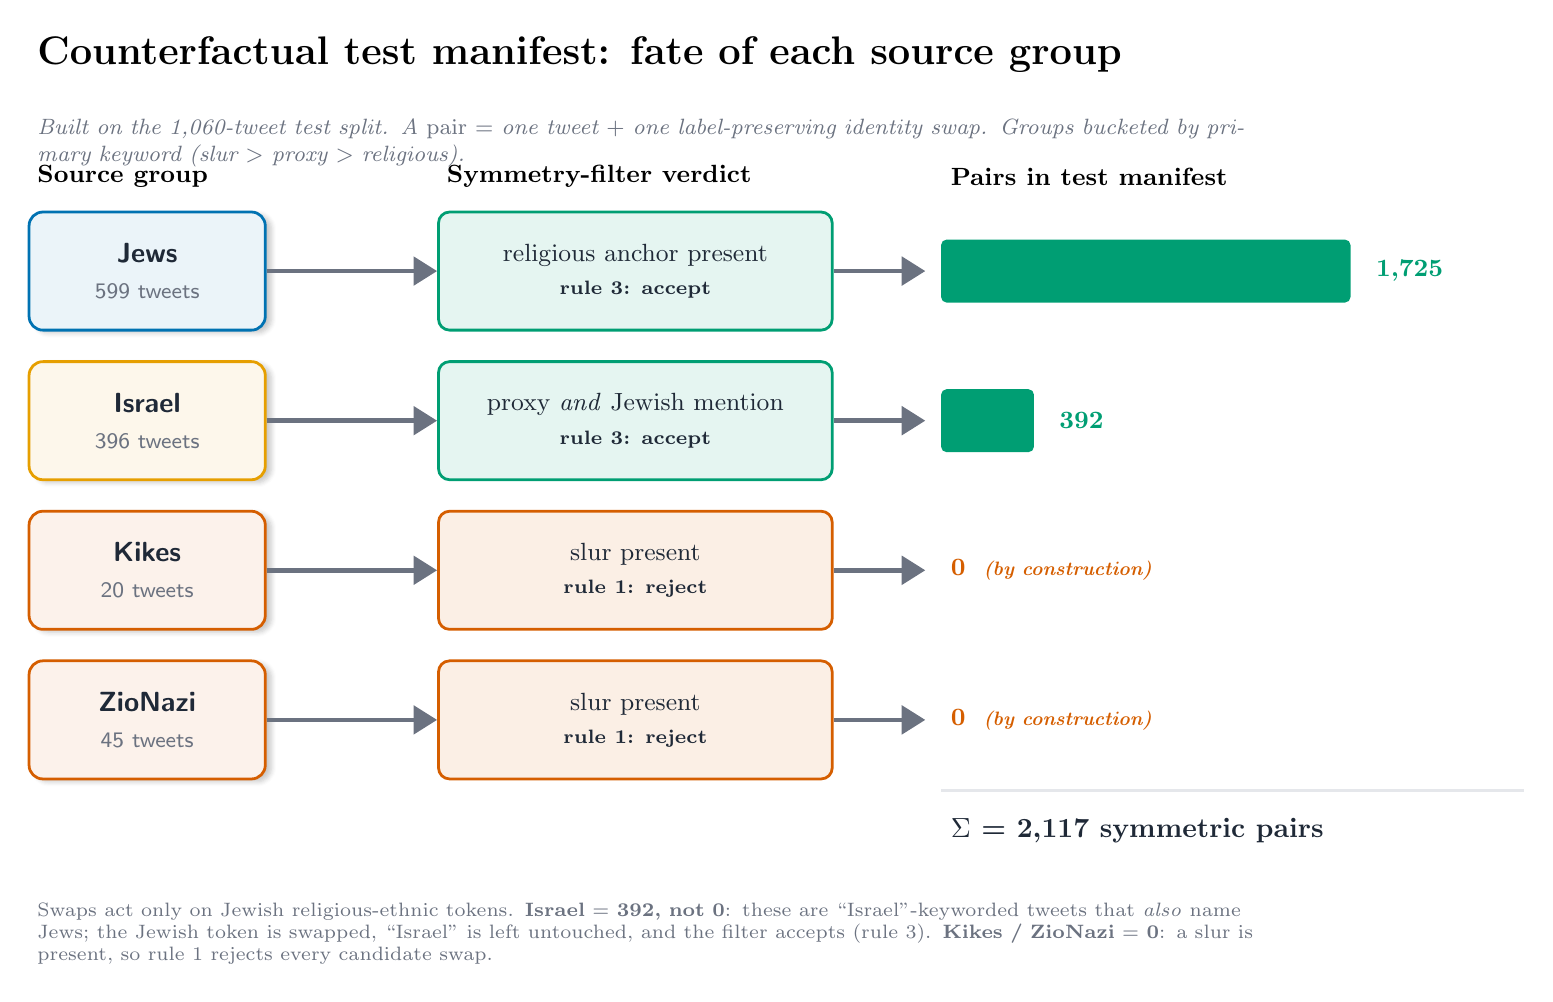
\begin{tikzpicture}[
  font=\sffamily,
  >={Stealth[round]},
  grp/.style={
    rounded corners=5pt, draw=#1, line width=1pt, fill=#1!8,
    text=inkdark, align=center, inner sep=6pt,
    minimum width=30mm, minimum height=15mm,
    blur shadow={shadow blur steps=5, shadow yshift=-1pt, shadow opacity=22}
  },
  verdict/.style={
    rounded corners=4pt, draw=#1, line width=1pt, fill=#1!10,
    text=inkdark, align=center, inner sep=5pt,
    minimum width=50mm, minimum height=15mm, font=\small
  },
  ar/.style={-{Triangle[length=3mm,width=3.6mm]}, line width=1.6pt, draw=slate},
]

% column anchors (x)
\def\GX{0mm}\def\VX{52mm}\def\BX{116mm}

% row y-coordinates
\def\yA{0mm}\def\yB{-19mm}\def\yC{-38mm}\def\yD{-57mm}

% ---------- column headers ----------
\node[font=\bfseries\small, anchor=west] at (\GX, 12mm) {Source group};
\node[font=\bfseries\small, anchor=west] at (\VX, 12mm) {Symmetry-filter verdict};
\node[font=\bfseries\small, anchor=west] at (\BX, 12mm) {Pairs in test manifest};

% =========================== ROW A: Jews ===========================
\node[grp=jewsc, anchor=west] (gA) at (\GX,\yA)
  {\textbf{Jews}\\[1pt]{\footnotesize\textcolor{slate}{599 tweets}}};
\node[verdict=accept, anchor=west] (vA) at (\VX,\yA)
  {religious anchor present\\[1pt]{\scriptsize\textbf{rule 3: accept}}};
\draw[ar] (gA.east) -- (vA.west);
\draw[ar] (vA.east) -- ([xshift=-2mm]\BX,\yA);
\fill[accept, rounded corners=2pt] (\BX,{\yA-4mm}) rectangle ($(\BX,{\yA+4mm})+(52mm,0)$);
\node[anchor=west, font=\small\bfseries, text=accept] at ($(\BX,\yA)+(54mm,0)$) {1{,}725};

% =========================== ROW B: Israel =========================
\node[grp=isrc, anchor=west] (gB) at (\GX,\yB)
  {\textbf{Israel}\\[1pt]{\footnotesize\textcolor{slate}{396 tweets}}};
\node[verdict=accept, anchor=west] (vB) at (\VX,\yB)
  {proxy \emph{and} Jewish mention\\[1pt]{\scriptsize\textbf{rule 3: accept}}};
\draw[ar] (gB.east) -- (vB.west);
\draw[ar] (vB.east) -- ([xshift=-2mm]\BX,\yB);
\fill[accept, rounded corners=2pt] (\BX,{\yB-4mm}) rectangle ($(\BX,{\yB+4mm})+(11.8mm,0)$);
\node[anchor=west, font=\small\bfseries, text=accept] at ($(\BX,\yB)+(13.8mm,0)$) {392};

% =========================== ROW C: Kikes ==========================
\node[grp=reject, anchor=west] (gC) at (\GX,\yC)
  {\textbf{Kikes}\\[1pt]{\footnotesize\textcolor{slate}{20 tweets}}};
\node[verdict=reject, anchor=west] (vC) at (\VX,\yC)
  {slur present\\[1pt]{\scriptsize\textbf{rule 1: reject}}};
\draw[ar] (gC.east) -- (vC.west);
\draw[ar] (vC.east) -- ([xshift=-2mm]\BX,\yC);
\node[anchor=west, font=\small\bfseries, text=reject] at (\BX,\yC)
  {0 \;{\scriptsize\itshape (by construction)}};

% =========================== ROW D: ZioNazi ========================
\node[grp=reject, anchor=west] (gD) at (\GX,\yD)
  {\textbf{ZioNazi}\\[1pt]{\footnotesize\textcolor{slate}{45 tweets}}};
\node[verdict=reject, anchor=west] (vD) at (\VX,\yD)
  {slur present\\[1pt]{\scriptsize\textbf{rule 1: reject}}};
\draw[ar] (gD.east) -- (vD.west);
\draw[ar] (vD.east) -- ([xshift=-2mm]\BX,\yD);
\node[anchor=west, font=\small\bfseries, text=reject] at (\BX,\yD)
  {0 \;{\scriptsize\itshape (by construction)}};

% ---------- total ----------
\draw[rail, line width=1pt] (\BX,{\yD-9mm}) -- ($(\BX,{\yD-9mm})+(74mm,0)$);
\node[anchor=west, font=\bfseries, text=inkdark] at (\BX,{\yD-14mm})
  {$\Sigma$ = 2{,}117 symmetric pairs};

% ---------- title ----------
\node[font=\bfseries\Large, anchor=south west] at (\GX, 24mm)
  {Counterfactual test manifest: fate of each source group};
\node[font=\itshape\footnotesize, text=slate, anchor=north west, text width=158mm] at (\GX, 20.5mm)
  {Built on the 1{,}060-tweet test split. A \emph{pair} $=$ one tweet $+$ one label-preserving identity swap. Groups bucketed by primary keyword (slur $>$ proxy $>$ religious).};

% ---------- footnote ----------
\node[font=\scriptsize, text=slate, anchor=north west, text width=158mm]
  at (\GX,{\yD-22mm})
  {Swaps act only on Jewish religious-ethnic tokens.
   \textbf{Israel $=$ 392, not 0}: these are ``Israel''-keyworded tweets that \emph{also} name Jews;
   the Jewish token is swapped, ``Israel'' is left untouched, and the filter accepts (rule 3).
   \textbf{Kikes / ZioNazi $=$ 0}: a slur is present, so rule 1 rejects every candidate swap.};

\end{tikzpicture}
\end{document}
